%% bare_conf.tex
%% V1.4b
%% 2015/08/26
%% by Michael Shell
%% See:
%% http://www.michaelshell.org/
%% for current contact information.
%%
%% This is a skeleton file demonstrating the use of IEEEtran.cls
%% (requires IEEEtran.cls version 1.8b or later) with an IEEE
%% conference paper.
%%
%% Support sites:
%% http://www.michaelshell.org/tex/ieeetran/
%% http://www.ctan.org/pkg/ieeetran
%% and
%% http://www.ieee.org/

%%*************************************************************************
%% Legal Notice:
%% This code is offered as-is without any warranty either expressed or
%% implied; without even the implied warranty of MERCHANTABILITY or
%% FITNESS FOR A PARTICULAR PURPOSE! 
%% User assumes all risk.
%% In no event shall the IEEE or any contributor to this code be liable for
%% any damages or losses, including, but not limited to, incidental,
%% consequential, or any other damages, resulting from the use or misuse
%% of any information contained here.
%%
%% All comments are the opinions of their respective authors and are not
%% necessarily endorsed by the IEEE.
%%
%% This work is distributed under the LaTeX Project Public License (LPPL)
%% ( http://www.latex-project.org/ ) version 1.3, and may be freely used,
%% distributed and modified. A copy of the LPPL, version 1.3, is included
%% in the base LaTeX documentation of all distributions of LaTeX released
%% 2003/12/01 or later.
%% Retain all contribution notices and credits.
%% ** Modified files should be clearly indicated as such, including  **
%% ** renaming them and changing author support contact information. **
%%*************************************************************************




\documentclass[conference]{IEEEtran}



\usepackage{cite}   % CITATION PACKAGE
\usepackage{amsmath } % MATH PACKAGES
\usepackage{algorithmic} % SPECIALIZED LIST PACKAGES (for code)
\usepackage{array} % ALIGNMENT PACKAGES (for arrays and tables)
\usepackage{url} % PDF, URL AND HYPERLINK PACKAGES
\usepackage{subcaption}



% *** GRAPHICS RELATED PACKAGES ***
\ifCLASSINFOpdf
  % for PDF mode
  \usepackage[pdftex]{graphicx}
  % \graphicspath{{../pdf/}{../jpeg/}}
  \DeclareGraphicsExtensions{.pdf, .jpeg, .png, .eps}
\else
  % for DVI mode
  \usepackage[dvips]{graphicx}
  % \graphicspath{{../eps/}}
  \DeclareGraphicsExtensions{.eps}
\fi

% *** SUBFIGURE PACKAGES ***
%\ifCLASSOPTIONcompsoc
%  \usepackage[caption=false,font=normalsize,labelfont=sf,textfont=sf]{subfig}
%\else
%  \usepackage[caption=false,font=footnotesize]{subfig}
%\fi





% *** FLOAT PACKAGES ***
%
%\usepackage{fixltx2e}
% fixltx2e, the successor to the earlier fix2col.sty, was written by
% Frank Mittelbach and David Carlisle. This package corrects a few problems
% in the LaTeX2e kernel, the most notable of which is that in current
% LaTeX2e releases, the ordering of single and double column floats is not
% guaranteed to be preserved. Thus, an unpatched LaTeX2e can allow a
% single column figure to be placed prior to an earlier double column
% figure.
% Be aware that LaTeX2e kernels dated 2015 and later have fixltx2e.sty's
% corrections already built into the system in which case a warning will
% be issued if an attempt is made to load fixltx2e.sty as it is no longer
% needed.
% The latest version and documentation can be found at:
% http://www.ctan.org/pkg/fixltx2e


%\usepackage{stfloats}
% stfloats.sty was written by Sigitas Tolusis. This package gives LaTeX2e
% the ability to do double column floats at the bottom of the page as well
% as the top. (e.g., "\begin{figure*}[!b]" is not normally possible in
% LaTeX2e). It also provides a command:
%\fnbelowfloat
% to enable the placement of footnotes below bottom floats (the standard
% LaTeX2e kernel puts them above bottom floats). This is an invasive package
% which rewrites many portions of the LaTeX2e float routines. It may not work
% with other packages that modify the LaTeX2e float routines. The latest
% version and documentation can be obtained at:
% http://www.ctan.org/pkg/stfloats
% Do not use the stfloats baselinefloat ability as the IEEE does not allow
% \baselineskip to stretch. Authors submitting work to the IEEE should note
% that the IEEE rarely uses double column equations and that authors should try
% to avoid such use. Do not be tempted to use the cuted.sty or midfloat.sty
% packages (also by Sigitas Tolusis) as the IEEE does not format its papers in
% such ways.
% Do not attempt to use stfloats with fixltx2e as they are incompatible.
% Instead, use Morten Hogholm'a dblfloatfix which combines the features
% of both fixltx2e and stfloats:
%
% \usepackage{dblfloatfix}
% The latest version can be found at:
% http://www.ctan.org/pkg/dblfloatfix






% *** Do not adjust lengths that control margins, column widths, etc. ***
% *** Do not use packages that alter fonts (such as pslatex).         ***



% correct bad hyphenation here
\hyphenation{op-tical net-works semi-conduc-tor}


\begin{document}


\title{Reverse Engineering Sound Modules}


% author names and affiliations
\author{
\IEEEauthorblockN{
  Anyere Bendrien\IEEEauthorrefmark{1},
  Adam Froghyar\IEEEauthorrefmark{2},
  Rodrigo Diaz\IEEEauthorrefmark{3} and
  Maximilian Wagenbach\IEEEauthorrefmark{4}
}
\IEEEauthorblockA{
  Audiocommunication Group\\
  Technical University of Berlin\\
  Einsteinufer 17, 10587 Berlin\\
}
\IEEEauthorblockA{\IEEEauthorrefmark{1}Email: anyere.bendrien@campus.tu-berlin.de}
\IEEEauthorblockA{\IEEEauthorrefmark{2}Email: 
a.froghyar@campus.tu-berlin.de}
\IEEEauthorblockA{\IEEEauthorrefmark{3}Email: rodrigodzf@gmail.com}
\IEEEauthorblockA{\IEEEauthorrefmark{4}Email: m.wagenbach@campus.tu-berlin.de}
}




% make the title area
\maketitle

% Abstract
\begin{abstract}
The sound of synthesizers based on analog circuits with their individual behavior and unique character generate a huge amount of fascination since the 60's.
Since the digital age there are respective digital sound modules generating an almost clean sound which is somewhat deterministic and therefore more predictable then their fellow analog campaigners.
The field of machine learning and advances in neural networks have received a lot of attention over the last years and today their application surrounds our everyday life.
There has been some research in how to use the same techniques for the purpose of expressing creativity.
This paper is a proof of concept that machine learning techniques can be used to synthesize sound with the thought of bringing some kind of \textit{analog} flair into the domain of digital sound processing.
With this research we take a dive in the vast field of neural networks.
\end{abstract}

% Keywords
\begin{IEEEkeywords}
  waveform, sound, recurrent neural network, long short term memory
\end{IEEEkeywords}



\section{Introduction}
During recent years the field of machine learning and artificial intelligence has gotten a lot of attention.
With the abundance of computing power, fast and cheap storage media, development of new algorithms as well as vast amount of data a lot of progress has been made.
Especially the fields of classification and recommendation have seen huge improvements due to artificial intelligence.
Even though most people do not realize it, today machine learning is already part of our day to day life.
Search engines and social networks use machine learning techniques for image recognition to categorize images, recognize faces or gather information that where previously unavailable for extraction by a computer.
Applying artificial intelligence techniques current smart-phones use voice recognition trained specifically to the voice of its owner to execute command.
In the automotive industry the upcoming self driving cars rely entirely on machine learning powered computer vision.
Today nearly every technology field tries to use "Big Data" to find useful correlations in unimaginable large data sets.

A few advances in machine learning have made its way into technology fields focused on creativity.
The usual classification techniques for example can of course easily be applied to classifying drum samples \cite{Herrera:DrumClassif} and organize large sound databases.
In 2015 \textit{Google} demonstrated that their deep neural network for image recognition \cite{GoogleDeepDream} could be used for a process they called "deep dreaming" which alienates images in an almost psychedelic way.
One example of a more domain specific use of artificial intelligence in digital audio technology namely music information retrieval is the use of a neural network to detect the onsets in a piece of music \cite{EybenOnSet} which can be used to calculate the beats per minute.


Very few efforts have been made to try to adapt the current research into a way of artistic expression.
The field of music synthesis has remained relatively untouched by the advances in artificial intelligence.
In this paper we want to outline our learning approach in trying to apply machine learning to music synthesis.
For this purpose, our goal is to train a neural network so that it can learn to emulate an oscillator.


\section{Related Work}

Using methods of artificial intelligence for music synthesis is a new and emerging field.
This reflects itself in the fact that there are very few published scientific papers on this subject.
The idea however to use neural networks for music synthesis is not new.
Concepts for it date back to the first rise in interest in the field of machine learning during the early 1990s.
Back then ideas and concepts where already developed, but the algorithms had not matured enough and computational power was simply not available at a reasonable cost.
There were however plans to realize a neural network audio synthesizer using dedicated hardware \cite{holler93}.
The need for purpose built hardware has disappeared today as the required memory and CPU power to run it in software on a general purpose computer is available today at a relatively low cost.

The current industry focus in artificial intelligence for audio synthesis lies in the field of speech synthesis.
This has many applications for the audio feedback of smartphones or so called "smart assistances".
One of the recent most notable examples is the development of WaveNet\footnote{\url{}https://deepmind.com/blog/wavenet-generative-model-raw-audio/} a convolutional neural network for speech synthesis by Google \cite{wavenet16}.
A small research group called Magenta within Google is researching the possibility to use state of the art neural networks for generating music and art in general.
They have recently published a synthesizer called NSynth\footnote{\url{https://magenta.tensorflow.org/nsynth}} based on WaveNet.
NSynth is able to generate sounds with the timbre of different instruments like for example Base, Organ, Glockenspiel or Flute sounds \cite{EngelRRDESN17}.
% Besides big tech cooperations there are also a few small startups that try different approaches to apply neural networks to sound and music generation.
% Unfortunately none of them have published any papers with advances they might have made.
% --> Wich corporations/statups? <--




\section{Recurrent Neural Networks}
As a starting point a special type of artificial neural network called recurrent neural networks (RNNs) was considered. Unlike standard fixed-sized input neurons, recurrent neural networks work with sequences of \textit{arbitrary} length, such as sentences, documents and audio samples as input.
Research has shown that recurrent neural networks have been quite successful in anticipating and exhibiting dynamic temporal behavior \cite{magenta} based on the fact that these neurons receive their own outputs as the input during the forthcoming frames. 
This type of behavior creates complex activation flows within the cells with more refined control over parameters, making RNNs a finer candidate than simple straightforward artificial networks. 
%\subsection{Recurrent Neural Networks}
\begin{figure}[h]
  \centering
  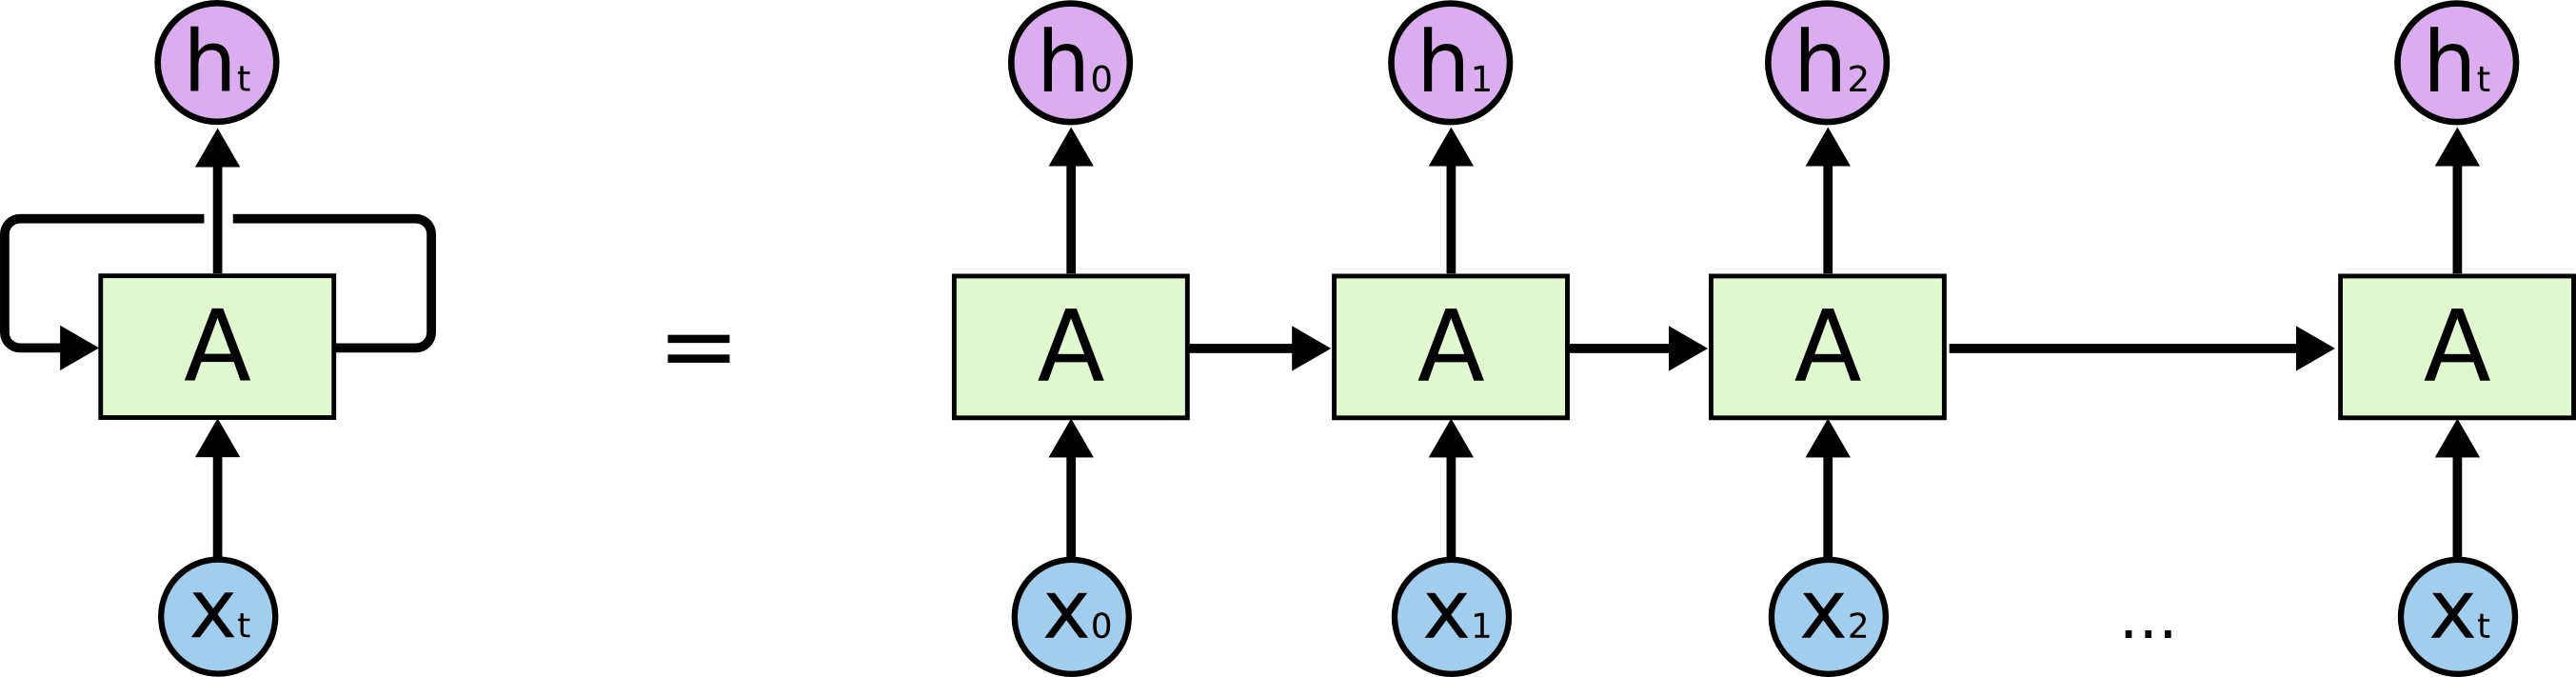
\includegraphics[width=3.2in]{Images/RNN-unrolled}
  \caption{\textit{Unrolling} a recurrent neuron}
  \label{unrolling}
\end{figure}
Figure \ref{unrolling} shows a typical recurrent neural network unrolled, revealing the backward pointing connections indicating the recurrence of previous outputs ($h_i$) as new inputs ($x_i$) \cite{colah}. The following equation describes the fundamentals of this behaviour
\begin{equation}
    \textbf{H}_{(t)} = \phi(\textbf{X}_{(t)}^T \cdot \textbf{W}_x  + \textbf{H}_{(t-1)}^T \cdot \textbf{W}_y +b),
\end{equation}
where the vectorized output $\textbf{H}_{(t)}$ at time-frame $t$ is a weighted relationship between vectorized inputs $\textbf{X}_{(t)}$ and previous outputs $\textbf{H}_{(t-1)}$ with bias term $b$, channeled through an either sigmoid \textit{tanh} or rectified linear unit $\phi$ activation function. The recurring nature of the system is apparent: $\textbf{H}_{(t)}$ is a function of $\textbf{X}_{(t)}$ and $\textbf{H}_{(t-1)}$, while $\textbf{H}_{(t-1)}$ is a function of $\textbf{X}_{(t-1)}$ and $\textbf{H}_{(t-2)}$ and so on - this makes $\textbf{H}_{(t)}$ a function of all inputs since $t=0$, as at the first time step the previous outputs are assumed to be all zeros. 

In artificial neural network terms, a part of a cell that preserves some state across time-frames is called a \textit{memory cell}. This notion of memory in the system has significantly different uses based on the desired outcome - parts of input and output sequences can be ignored so that only one vector of outputs is produced from a sequence of input vectors and vice versa. In the case of modeling a continuously sampled audio signal (be it speech or the characteristics of an analogue filter), a \textit{sequence to sequence} approach is applicable, where a sequence of inputs is generating a sequence of outputs. 
\subsection{Long Short Term Memory}
Introduced in 1997 by Hochreiter and Schmidhuber, Long Short Term Memory (LSTM) is a special type of RNN that can detect long-term dependencies in data by learning to bridge minimal time lags in excess of 1000 discrete time steps by enforcing constant error flows within special units of data \cite{LSTM}. This means that while simple RNNs do possess memory in their network, the higher the gap between the two pieces of information that need to be matched, the more likely it is for the RNN to fail - a LSTM cell bridges this gap by splitting its state vectors into \textit{short-term} and \textit{long-term} states. LSTM neural networks have also been used successfully  in the past for speech synthesis \cite{LSTMspeech_ChungKDGCB15}, so a new implication of this recurrent neural network on different types of audio data has been a motivating factor behind this research.
\begin{figure}[h]
  \centering
  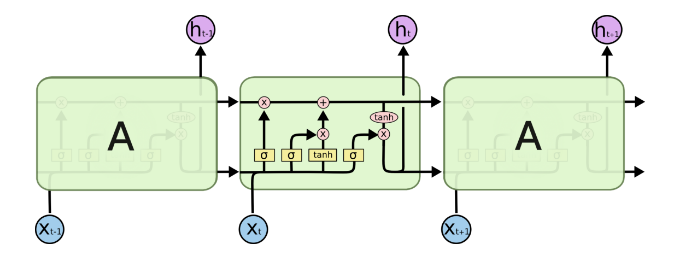
\includegraphics[width=3.5in]{Images/LSTM}
  \caption{Repeating, interacting \textit{LSTM} modules}
  \label{LSTM}
\end{figure}
\\
Figure \ref{LSTM} above represents multiple LSTM neurons interacting with each other, where the different memory states \textit{traverse} through the cell and interact with the information gained from previous states \cite{colah}. The key idea of this algorithm is that the network can learn what to store in the long-term state, what to throw away and what to read from it. The way the algorithm decides what information is passed through from one state to another is through \textit{gates}, which are optional information filtering operations composed of a sigmoid neural layer (outputting numbers between 0 and 1 - i.e. 'let nothing/everything in') and point-wise multiplication.

The \textit{Long-term state} traverses from left to right on the top, passing through two gates, the first of which is a multiplicative \textit{forget-gate} dropping memories followed by an additive operation of implementing new memories into the long-term memory of the network with the previous short-term state $h_{t-1}$ and the new input sample $x_t$ being the sources of information. 

The \textit{Short-term state} traverses on the bottom of the cell representation with constant connection to the long-term state through sigmoid gating signals and hyperbolic tangent activation functions. As seen on figure \ref{longshort}, the previous cell's short term state $h_{t-1}$ and the new input sample $x_t$ is gated by the first sigmoid layer to decide what \textit{percentage} of the information is to be passed into the current long-term state \cite{colah}. The second sigmoid layer multiplied with the \textit{tanh} activation function then defines the
\textit{new candidate values} scaled by how much we decided to update each state value.
\begin{figure}[h]
\begin{subfigure}{.25\textwidth}
  \centering
  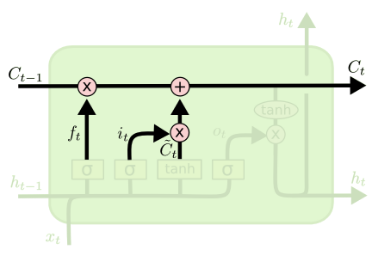
\includegraphics[width=.8\linewidth]{Images/4}
%   \caption{}
  \label{fig:sfig1}
\end{subfigure}%
\begin{subfigure}{.25\textwidth}
   \centering
  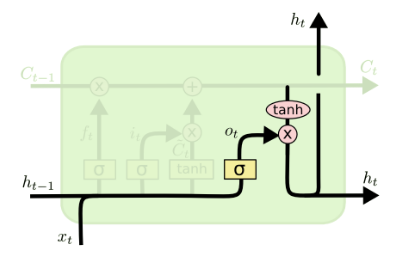
\includegraphics[width=.8\linewidth]{Images/5}
%   \caption{1b}
  \label{fig:sfig2}
\end{subfigure}
\caption{Long-term (left) and short-term (right) states within a LSTM cell}
\label{longshort}
\end{figure}

The old cell state $C_{t-1}$ (i.e. the long term state traversing on the top of the diagram) now needs to be updated to the new cell state $C_t$, an output of this time frame $h_t$ needs to be produced and an updated strain of short-term information needs to be sent into the next cell state. 

The previous long-term cell state $C_{t-1}$ updated by the gated functions $f_t$ and $i_t \times \tilde{C}_t$ now includes all the updated information we have let through from the previous short term state and new input information, and is now - by the multiplication and addition operations - updated to the current long-term state $C_t$ that is being sent into the next frame's cell. 

The algorithm's complex definition of the network's long-term memory strongly relies on using predefined gates and activation functions to influence what type of information is "mixed in" form the short-term memory and new input values - this dependency is also apparent in the cell's actual output, i.e. defining what exactly we store in the \textit{short-term} memory based on previous short-, and long-term states and the frame's new input sample. 

The actual output of the cell goes through another filtering layer before $h_{t-1}$ is updated to $h_t$. Another sigmoid layer decides which part of the previous short-term state and new sample is pushed forward by $o_t$, which is then multiplied by the \textit{tanh} activated long-term state that we have decided to include in the new short-term state and output of the cell.

This complex interdependency of short and long-term states in the definition of the different output layers of these LSTM cells gives rise to a highly definable set of gates and activation functions that reiteratively correct error data and are also adjustable for different implications by the user. The fact that the algorithm reacts immediately to new samples and predefined shor-term memory information as well as constantly updating and implementing a set of long-term memory information makes the LSTM neural network a highly usable algorithm for our desired implication of modeling a continuous signal of audio data with abrupt short-term signal changes as well as long-term progressions in the frequency spectra.

\section{What we did}

There are numerous open-source machine learning tools that include parameterizable RNN models, including LSTM. We opted for Keras\footnote{\url{https://keras.io/}} a machine learning library written in Python. Keras offers a high-level API that uses TensorFlow \footnote{\url{https://www.tensorflow.org/}} or Theano\footnote{\url{https://github.com/Theano/Theano}} as a back-end.

First, we produced a synthetic dataset composed of different sample signals, including a sine, square and sawtooth waves. We used 1024 samples per sample signal. Since LSTM accepts an input-output sequence at a time, we pre-processed each dataset by grouping each two consecutive samples (within the sample signal) as an input and an output datasets.

After this we train the LSTM layer with 2 units. Due to the batch size, which is equal to the size of the dataset, we do not need a stateful LSTM. The model is built using the mean square error (MSE) as the loss function and stochastic optimization (ADAM).

A second LSTM model with an auxiliary input for the corresponding frequencies of each sample signal is also used. Like in the first model this one is also optimized using ADAM and uses mean square error as the loss function.

% The performance of the model in both cases is measured using root mean square error (RMSE) between the predicted values and the original signal.

\section{Evaluation}

Given the simplicity of the dataset i.e., a periodic sine, square and sawtooth, the training RMSE when predicting the original waveform is minimal (in most cases below 0.2). We do not use a proper validation or test datasets, however we evaluate the performance of our model based on its ability to predict consecutive values. That is, given a first sample, the model will use the predicted value for the first sample, to predict a third sample and so forth. This generated signal is compared to the original signal for each of our sample signals (see Table \ref{tab:err}).

% we do not use  validation set, however we use the generative signal as a performance metric 

% sine
% Train Score (less is better): 0.14 RMSE
% generative RMSE 0.46

% saw 
% Train Score (less is better): 0.16 RMSE
% RMSE 0.34

% square
% Train Score (less is better): 0.24 RMSE
% RMSE 0.62

\begin{table}[!t]
  %% increase table row spacing, adjust to taste
  \renewcommand{\arraystretch}{1.4}
  \caption{Error estimation of three trained models}
  \label{tab:err}
  \centering
  \begin{tabular}{|c|c|c|}
    \hline
    Waveform & Training RMSE & Generative RMSE \\
    \hline
    Sine & 0.14 & 0.46 \\
    \hline
    Sawtooth & 0.16 & 0.34 \\
    \hline
    Square & 0.24 & 0.62 \\
    \hline
  \end{tabular}
\end{table}

However, our model generally overfits the data because it does not respond well to changes in amplitude or frequency. Nor is it able to predict correctly the next values based on previous output values, meaning that the relationship between consecutive samples has not been correctly learned. A bigger dataset seems to have little effect on the results. In fact, it is reasonable to use only one period since the waveform is periodic.

% This is not true because I couldn't get the auxiliary input to work yet!!!!!
% MAYBE DELETE THIS??
%The model using an auxiliary input responds better since it relies on extra information for predicting each value. 
%This is similar to produce a model for each waveform with a particular frequency.

% SEE Table
Predicting the sine and the sawtooth waveforms seem to perform better than the square as well (see figure \ref{fig:waveforms}).
% However the LSTM model performs better if a state

\begin{figure}[!t]
\begin{subfigure}{0.5\textwidth}
  \centering
  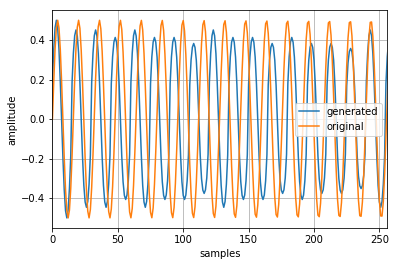
\includegraphics[width=.8\linewidth]{Images/sine_gen}
  \caption{Sine}
  \label{fig:sfig1}
\end{subfigure}
\begin{subfigure}{0.5\textwidth}
  \centering
  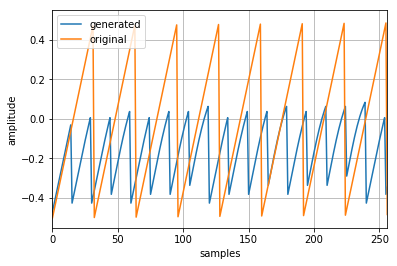
\includegraphics[width=.8\linewidth]{Images/saw_gen}
  \caption{Sawtooth}
  \label{fig:sfig2}
\end{subfigure}
\begin{subfigure}{0.5\textwidth}
  \centering
  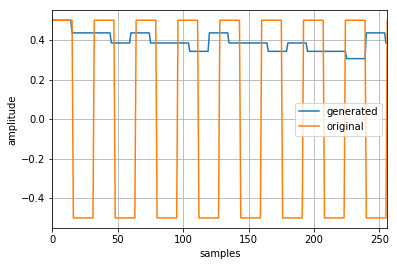
\includegraphics[width=.8\linewidth]{Images/square_gen}
  \caption{Square}
  \label{fig:sfig3}
\end{subfigure}
\caption{Waveforms of original and generated signals}
\label{fig:waveforms}
\end{figure}

\section{Conclusion and Future Work}
We were able to train neural networks emulating common waveforms with the use of LSTM.
Especially the sine and sawtooth models got exciting results.
Our trained model on more abrupt changing waveforms like a square wave is not as accurate as the other models though it still provides recognizable results.

LSTM is intuitively a good alternative to learn waveforms, however other models such as CNN, might outperform LSTM with simple datasets.
We were not able to address an overfitting in our models, this can be improved in further research using layered LSTMs, more complex architectures, and longer learning sequences.
It remains to be seen, if our LSTM model can handle other waveforms. Different types of RNN architectures that have been used for speech synthesis\cite{wu2016merlin} can also be used to learn simple waveforms.

% use section* for acknowledgment
\section*{Acknowledgment}

We would like to thank Athanasios Lykartsis for assistance in writing up this paper as well as introducing us to the field of machine learning.



% An example of a floating figure using the graphicx package.
% Note that \label must occur AFTER (or within) \caption.
% For figures, \caption should occur after the \includegraphics.
% Note that IEEEtran v1.7 and later has special internal code that
% is designed to preserve the operation of \label within \caption
% even when the captionsoff option is in effect. However, because
% of issues like this, it may be the safest practice to put all your
% \label just after \caption rather than within \caption{}.
%
% Reminder: the "draftcls" or "draftclsnofoot", not "draft", class
% option should be used if it is desired that the figures are to be
% displayed while in draft mode.
%
%\begin{figure}[!t]
%\centering
%\includegraphics[width=2.5in]{myfigure}
% where an .eps filename suffix will be assumed under latex, 
% and a .pdf suffix will be assumed for pdflatex; or what has been declared
% via \DeclareGraphicsExtensions.
%\caption{Simulation results for the network.}
%\label{fig_sim}
%\end{figure}

% Note that the IEEE typically puts floats only at the top, even when this
% results in a large percentage of a column being occupied by floats.


% An example of a double column floating figure using two subfigures.
% (The subfig.sty package must be loaded for this to work.)
% The subfigure \label commands are set within each subfloat command,
% and the \label for the overall figure must come after \caption.
% \hfil is used as a separator to get equal spacing.
% Watch out that the combined width of all the subfigures on a 
% line do not exceed the text width or a line break will occur.
%
%\begin{figure*}[!t]
%\centering
%\subfloat[Case I]{\includegraphics[width=2.5in]{box}%
%\label{fig_first_case}}
%\hfil
%\subfloat[Case II]{\includegraphics[width=2.5in]{box}%
%\label{fig_second_case}}
%\caption{Simulation results for the network.}
%\label{fig_sim}
%\end{figure*}
%
% Note that often IEEE papers with subfigures do not employ subfigure
% captions (using the optional argument to \subfloat[]), but instead will
% reference/describe all of them (a), (b), etc., within the main caption.
% Be aware that for subfig.sty to generate the (a), (b), etc., subfigure
% labels, the optional argument to \subfloat must be present. If a
% subcaption is not desired, just leave its contents blank,
% e.g., \subfloat[].


% An example of a floating table. Note that, for IEEE style tables, the
% \caption command should come BEFORE the table and, given that table
% captions serve much like titles, are usually capitalized except for words
% such as a, an, and, as, at, but, by, for, in, nor, of, on, or, the, to
% and up, which are usually not capitalized unless they are the first or
% last word of the caption. Table text will default to \footnotesize as
% the IEEE normally uses this smaller font for tables.
% The \label must come after \caption as always.
%
%\begin{table}[!t]
%% increase table row spacing, adjust to taste
%\renewcommand{\arraystretch}{1.3}
% if using array.sty, it might be a good idea to tweak the value of
% \extrarowheight as needed to properly center the text within the cells
%\caption{An Example of a Table}
%\label{table_example}
%\centering
%% Some packages, such as MDW tools, offer better commands for making tables
%% than the plain LaTeX2e tabular which is used here.
%\begin{tabular}{|c||c|}
%\hline
%One & Two\\
%\hline
%Three & Four\\
%\hline
%\end{tabular}
%\end{table}


% Note that the IEEE does not put floats in the very first column
% - or typically anywhere on the first page for that matter. Also,
% in-text middle ("here") positioning is typically not used, but it
% is allowed and encouraged for Computer Society conferences (but
% not Computer Society journals). Most IEEE journals/conferences use
% top floats exclusively. 
% Note that, LaTeX2e, unlike IEEE journals/conferences, places
% footnotes above bottom floats. This can be corrected via the
% \fnbelowfloat command of the stfloats package.







% trigger a \newpage just before the given reference
% number - used to balance the columns on the last page
% adjust value as needed - may need to be readjusted if
% the document is modified later
%\IEEEtriggeratref{8}
% The "triggered" command can be changed if desired:
%\IEEEtriggercmd{\enlargethispage{-5in}}

% references section

% can use a bibliography generated by BibTeX as a .bbl file
% BibTeX documentation can be easily obtained at:
% http://mirror.ctan.org/biblio/bibtex/contrib/doc/
% The IEEEtran BibTeX style support page is at:
% http://www.michaelshell.org/tex/ieeetran/bibtex/
%\bibliographystyle{IEEEtran}
% argument is your BibTeX string definitions and bibliography database(s)
%\bibliography{IEEEabrv,../bib/paper}
%
% <OR> manually copy in the resultant .bbl file
% set second argument of \begin to the number of references
% (used to reserve space for the reference number labels box)
%\begin{thebibliography}{1}


%\end{thebibliography}

\bibliographystyle{IEEEtran}
\bibliography{literature}


% that's all folks
\end{document}


